

\tikzset{every picture/.style={line width=0.75pt}} %set default line width to 0.75pt        

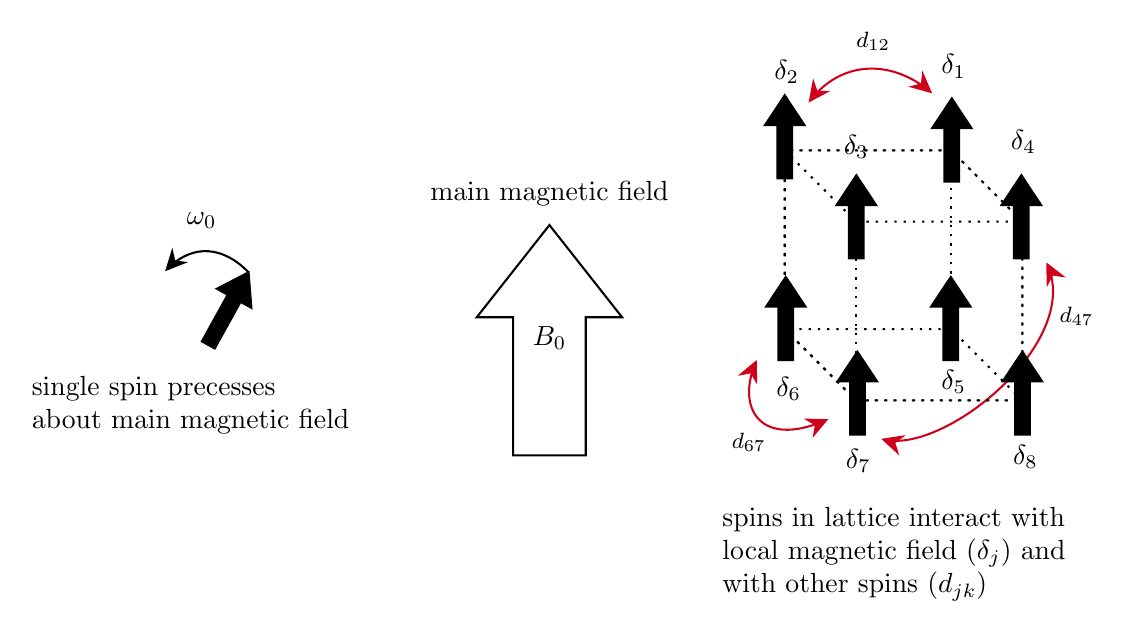
\begin{tikzpicture}[x=0.75pt,y=0.75pt,yscale=-1,xscale=1]
%uncomment if require: \path (0,379); %set diagram left start at 0, and has height of 379

%Up Arrow [id:dp7271723556391365] 
\draw  [fill={rgb, 255:red, 0; green, 0; blue, 0 }  ,fill opacity=1 ] (366.75,82.33) -- (376.25,68) -- (385.75,82.33) -- (379.78,82.33) -- (379.78,108) -- (372.72,108) -- (372.72,82.33) -- cycle ;
%Up Arrow [id:dp9463814628049166] 
\draw  [fill={rgb, 255:red, 0; green, 0; blue, 0 }  ,fill opacity=1 ] (401.25,120.83) -- (410.75,106.5) -- (420.25,120.83) -- (414.28,120.83) -- (414.28,146.5) -- (407.22,146.5) -- (407.22,120.83) -- cycle ;
%Up Arrow [id:dp31057152898577745] 
\draw  [fill={rgb, 255:red, 0; green, 0; blue, 0 }  ,fill opacity=1 ] (447.25,83.83) -- (456.75,69.5) -- (466.25,83.83) -- (460.28,83.83) -- (460.28,109.5) -- (453.22,109.5) -- (453.22,83.83) -- cycle ;
%Curve Lines [id:da4975212833523538] 
\draw [color={rgb, 255:red, 208; green, 2; blue, 27 }  ,draw opacity=1 ]   (361.47,198.59) .. controls (353.57,219.73) and (365.13,237.42) .. (394.92,225.01) ;
\draw [shift={(397.25,224)}, rotate = 515.56] [fill={rgb, 255:red, 208; green, 2; blue, 27 }  ,fill opacity=1 ][line width=0.08]  [draw opacity=0] (10.72,-5.15) -- (0,0) -- (10.72,5.15) -- (7.12,0) -- cycle    ;
\draw [shift={(362.75,195.5)}, rotate = 114.54] [fill={rgb, 255:red, 208; green, 2; blue, 27 }  ,fill opacity=1 ][line width=0.08]  [draw opacity=0] (10.72,-5.15) -- (0,0) -- (10.72,5.15) -- (7.12,0) -- cycle    ;
%Curve Lines [id:da3784526253823667] 
\draw [color={rgb, 255:red, 208; green, 2; blue, 27 }  ,draw opacity=1 ]   (425.99,234.21) .. controls (456.35,238.48) and (518.05,186.82) .. (503.25,150.69) ;
\draw [shift={(502.25,148.5)}, rotate = 423.13] [fill={rgb, 255:red, 208; green, 2; blue, 27 }  ,fill opacity=1 ][line width=0.08]  [draw opacity=0] (10.72,-5.15) -- (0,0) -- (10.72,5.15) -- (7.12,0) -- cycle    ;
\draw [shift={(422.75,233.5)}, rotate = 16.97] [fill={rgb, 255:red, 208; green, 2; blue, 27 }  ,fill opacity=1 ][line width=0.08]  [draw opacity=0] (10.72,-5.15) -- (0,0) -- (10.72,5.15) -- (7.12,0) -- cycle    ;
%Curve Lines [id:da8584645943617881] 
\draw [color={rgb, 255:red, 208; green, 2; blue, 27 }  ,draw opacity=1 ]   (389.6,69.13) .. controls (404.14,51.68) and (426.64,50.73) .. (444.98,65.12) ;
\draw [shift={(447.25,67)}, rotate = 221.07999999999998] [fill={rgb, 255:red, 208; green, 2; blue, 27 }  ,fill opacity=1 ][line width=0.08]  [draw opacity=0] (10.72,-5.15) -- (0,0) -- (10.72,5.15) -- (7.12,0) -- cycle    ;
\draw [shift={(387.75,71.5)}, rotate = 306.19] [fill={rgb, 255:red, 208; green, 2; blue, 27 }  ,fill opacity=1 ][line width=0.08]  [draw opacity=0] (10.72,-5.15) -- (0,0) -- (10.72,5.15) -- (7.12,0) -- cycle    ;
%Up Arrow [id:dp3158905830854031] 
\draw  [fill={rgb, 255:red, 0; green, 0; blue, 0 }  ,fill opacity=1 ] (480.75,120.83) -- (490.25,106.5) -- (499.75,120.83) -- (493.78,120.83) -- (493.78,146.5) -- (486.72,146.5) -- (486.72,120.83) -- cycle ;
%Up Arrow [id:dp36356262031151887] 
\draw  [fill={rgb, 255:red, 0; green, 0; blue, 0 }  ,fill opacity=1 ] (367.25,169.83) -- (376.75,155.5) -- (386.25,169.83) -- (380.28,169.83) -- (380.28,195.5) -- (373.22,195.5) -- (373.22,169.83) -- cycle ;
%Up Arrow [id:dp766389940315232] 
\draw  [fill={rgb, 255:red, 0; green, 0; blue, 0 }  ,fill opacity=1 ] (401.75,205.83) -- (411.25,191.5) -- (420.75,205.83) -- (414.78,205.83) -- (414.78,231.5) -- (407.72,231.5) -- (407.72,205.83) -- cycle ;
%Up Arrow [id:dp2049142247539446] 
\draw  [fill={rgb, 255:red, 0; green, 0; blue, 0 }  ,fill opacity=1 ] (446.75,169.83) -- (456.25,155.5) -- (465.75,169.83) -- (459.78,169.83) -- (459.78,195.5) -- (452.72,195.5) -- (452.72,169.83) -- cycle ;
%Up Arrow [id:dp10669917595785261] 
\draw  [fill={rgb, 255:red, 0; green, 0; blue, 0 }  ,fill opacity=1 ] (481.25,205.83) -- (490.75,191.5) -- (500.25,205.83) -- (494.28,205.83) -- (494.28,231.5) -- (487.22,231.5) -- (487.22,205.83) -- cycle ;
%Shape: Cube [id:dp519829571353126] 
\draw  [dash pattern={on 0.84pt off 2.51pt}] (490.75,128.85) -- (456.4,94.5) -- (376.25,94.5) -- (376.25,180.65) -- (410.6,215) -- (490.75,215) -- cycle ; \draw  [dash pattern={on 0.84pt off 2.51pt}] (376.25,94.5) -- (410.6,128.85) -- (490.75,128.85) ; \draw  [dash pattern={on 0.84pt off 2.51pt}] (410.6,128.85) -- (410.6,215) ;
%Shape: Cube [id:dp8425873852655799] 
\draw  [dash pattern={on 0.84pt off 2.51pt}] (376.25,180.65) -- (410.6,215) -- (490.75,215) -- (490.75,128.85) -- (456.4,94.5) -- (376.25,94.5) -- cycle ; \draw  [dash pattern={on 0.84pt off 2.51pt}] (490.75,215) -- (456.4,180.65) -- (376.25,180.65) ; \draw  [dash pattern={on 0.84pt off 2.51pt}] (456.4,180.65) -- (456.4,94.5) ;


%Up Arrow [id:dp61739897786365] 
\draw   (227.88,174.9) -- (262.88,130.5) -- (297.88,174.9) -- (280.38,174.9) -- (280.38,241.5) -- (245.38,241.5) -- (245.38,174.9) -- cycle ;


%Up Arrow [id:dp98446138321537] 
\draw  [fill={rgb, 255:red, 0; green, 0; blue, 0 }  ,fill opacity=1 ] (102.66,161.19) -- (117.92,153.26) -- (119.28,170.4) -- (114.06,167.5) -- (101.61,189.95) -- (95.44,186.53) -- (107.88,164.08) -- cycle ;
%Curve Lines [id:da20736812223046341] 
\draw    (117.92,153.26) .. controls (105.45,140.49) and (91.37,139.79) .. (79.73,150.72) ;
\draw [shift={(77.72,152.75)}, rotate = 312.71000000000004] [fill={rgb, 255:red, 0; green, 0; blue, 0 }  ][line width=0.08]  [draw opacity=0] (10.72,-5.15) -- (0,0) -- (10.72,5.15) -- (7.12,0) -- cycle    ;



% Text Node
\draw (253.38,177.9) node [anchor=north west][inner sep=0.75pt]    {$B_{0}$};
% Text Node
\draw (349.25,229.4) node [anchor=north west][inner sep=0.75pt]  [font=\footnotesize]  {$d_{67}$};
% Text Node
\draw (507.25,168.4) node [anchor=north west][inner sep=0.75pt]  [font=\footnotesize]  {$d_{47}$};
% Text Node
\draw (409.25,35.9) node [anchor=north west][inner sep=0.75pt]  [font=\footnotesize]  {$d_{12}$};
% Text Node
\draw (369.75,49.4) node [anchor=north west][inner sep=0.75pt]    {$\delta _{2}$};
% Text Node
\draw (403.25,85.9) node [anchor=north west][inner sep=0.75pt]    {$\delta _{3}$};
% Text Node
\draw (450.25,46.9) node [anchor=north west][inner sep=0.75pt]    {$\delta _{1}$};
% Text Node
\draw (483.75,83.4) node [anchor=north west][inner sep=0.75pt]    {$\delta _{4}$};
% Text Node
\draw (370.75,202.4) node [anchor=north west][inner sep=0.75pt]    {$\delta _{6}$};
% Text Node
\draw (404.25,236.9) node [anchor=north west][inner sep=0.75pt]    {$\delta _{7}$};
% Text Node
\draw (450.25,198.9) node [anchor=north west][inner sep=0.75pt]    {$\delta _{5}$};
% Text Node
\draw (484.75,234.9) node [anchor=north west][inner sep=0.75pt]    {$\delta _{8}$};
% Text Node
\draw (262.88,115.5) node   [align=left] {main magnetic field};
% Text Node
\draw (86.72,123.15) node [anchor=north west][inner sep=0.75pt]    {$\omega _{0}$};
% Text Node
\draw (12,201.75) node [anchor=north west][inner sep=0.75pt]   [align=left] {single spin precesses\\about main magnetic field};
% Text Node
\draw (344.75,265) node [anchor=north west][inner sep=0.75pt]   [align=left] {spins in lattice interact with\\local magnetic field ($\displaystyle \delta _{j}$) and\\with other spins ($\displaystyle d_{jk}$)};


\end{tikzpicture}
